\chapter{THỬ NGHIỆM, KẾT QUẢ VÀ THẢO LUẬN}

\section{Thiết lập thí nghiệm}

Dữ liệu được chia như mục~\ref{sec:chia-du-lieu}; ảnh xám $32\times32$; \texttt{random\_state}=42 cho mọi bước ngẫu nhiên. Tiêu chí đánh giá gồm Accuracy, Macro-Precision, Macro-Recall, Macro-F1 (phù hợp với dữ liệu mất cân bằng), ma trận nhầm lẫn, chỉ số theo từng lớp, độ chính xác theo kích thước biển và thời gian huấn luyện, dự đoán.

\textbf{Phương án baseline.} Vector pixel $32\times32$ kết hợp K-NN ($k=5$, euclidean), không dùng CLAHE. Trên tập kiểm định baseline đạt Accuracy 0.5099 và Macro-F1 0.4187; trên tập Test đạt Accuracy \textbf{0.5253} và Macro-F1 \textbf{0.4682}. Mọi phương án khác được so sánh với mốc này.

\section{So sánh tiền xử lý CLAHE}
\label{sec:so-sanh-clahe}

Bảng~\ref{tab:clahe} so sánh việc dùng và không dùng CLAHE trên tập kiểm định, với K-NN ($k=5$) và Cây quyết định (tham số mặc định).

\begin{table}[H]
\centering
\caption{Ảnh hưởng của CLAHE trên tập kiểm định}
\label{tab:clahe}
\begin{tabular}{|p{3.6cm}|p{2.6cm}|p{2.2cm}|p{2.6cm}|p{2.6cm}|}
\hline
\textbf{Thuật toán} & \textbf{Biểu diễn} & \textbf{CLAHE} & \textbf{Accuracy} & \textbf{Macro-F1} \\
\hline
K-NN & Pixel & Không & 0.5099 & 0.4187 \\
\hline
K-NN & Pixel & Có & 0.6851 & 0.5996 \\
\hline
K-NN & HOG & Không & 0.9230 & 0.9067 \\
\hline
K-NN & HOG & Có & 0.9225 & 0.9113 \\
\hline
Cây quyết định & Pixel & Không & 0.6065 & 0.4997 \\
\hline
Cây quyết định & Pixel & Có & 0.6973 & 0.6006 \\
\hline
Cây quyết định & HOG & Không & 0.7794 & 0.7128 \\
\hline
Cây quyết định & HOG & Có & 0.7674 & 0.7014 \\
\hline
\end{tabular}
\Nguon{Nhóm tổng hợp từ tệp \texttt{results/validation\_results.csv}}
\end{table}

Với biểu diễn pixel, CLAHE tăng Macro-F1 rõ rệt (K-NN tăng 0.181; Cây quyết định tăng 0.101). Với HOG, tác động không nhất quán (K-NN tăng 0.005, Cây quyết định giảm 0.011). Theo quy tắc chọn, CLAHE được dùng cho biểu diễn pixel và không dùng cho HOG.

\section{Quét siêu tham số trên tập kiểm định}

Bảng~\ref{tab:cau-hinh-tot-nhat} là cấu hình tốt nhất của từng cặp (thuật toán, biểu diễn); Hình~\ref{fig:knn-k} cho thấy ảnh hưởng của $k$ và metric lên Macro-F1 của K-NN.

\begin{table}[H]
\centering
\caption{Cấu hình tốt nhất trên tập kiểm định (chọn theo Macro-F1)}
\label{tab:cau-hinh-tot-nhat}
\small
\begin{tabular}{|p{2.5cm}|p{2.3cm}|p{1.4cm}|p{3.6cm}|p{1.8cm}|p{1.9cm}|}
\hline
\textbf{Thuật toán} & \textbf{Biểu diễn} & \textbf{CLAHE} & \textbf{Tham số} & \textbf{Accuracy} & \textbf{Macro-F1} \\
\hline
K-NN & HOG & Không & $k=9$, euclidean & 0.9284 & 0.9103 \\
\hline
K-NN & PCA-HOG & Không & $k=7$, manhattan & 0.9165 & 0.8972 \\
\hline
K-NN & PCA-pixel & Có & $k=1$, manhattan & 0.7632 & 0.7160 \\
\hline
K-NN & Pixel & Có & $k=1$, euclidean & 0.6920 & 0.6171 \\
\hline
Cây quyết định & HOG & Không & độ sâu không giới hạn, gini & 0.7794 & 0.7128 \\
\hline
Cây quyết định & PCA-HOG & Không & độ sâu 20, entropy & 0.7256 & 0.6630 \\
\hline
Cây quyết định & Pixel & Có & độ sâu 20, entropy & 0.7204 & 0.6477 \\
\hline
Cây quyết định & PCA-pixel & Có & độ sâu 20, entropy & 0.5823 & 0.4768 \\
\hline
\end{tabular}
\Nguon{Nhóm tổng hợp từ tệp \texttt{results/best\_per\_config\_val.csv}}
\end{table}

\begin{figure}[H]
    \centering
    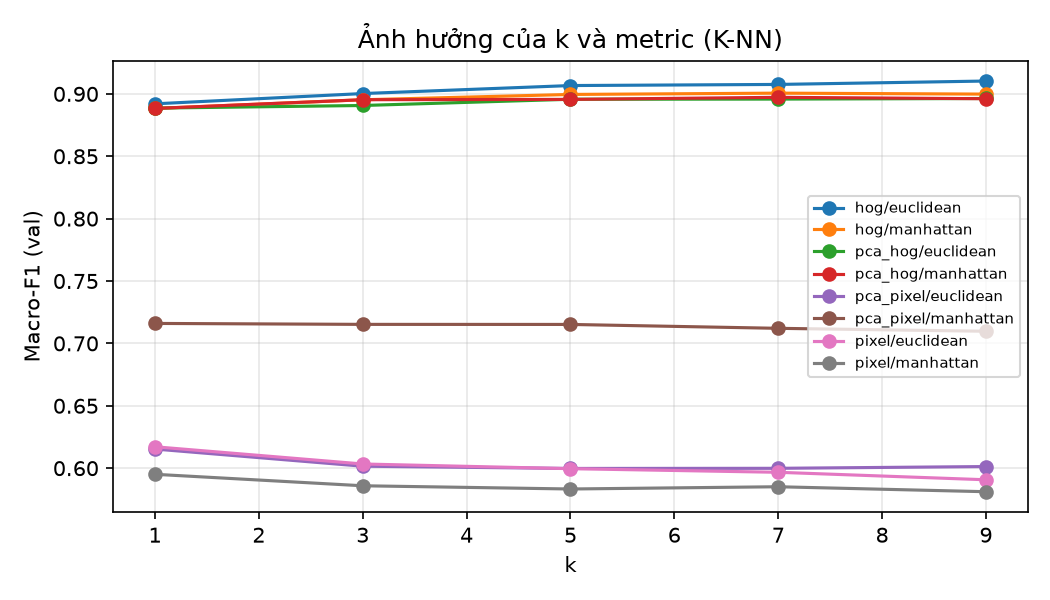
\includegraphics[width=0.8\textwidth]{images/fig_knn_k.png}
    \caption{Ảnh hưởng của $k$ và metric lên Macro-F1 trên tập kiểm định (K-NN)}
    \label{fig:knn-k}
    \Nguon{Nhóm vẽ từ kết quả thực nghiệm}
\end{figure}

\section{Kết quả cuối trên tập kiểm thử}

\begin{table}[H]
\centering
\caption{Kết quả trên tập Test (12\,630 ảnh)}
\label{tab:ket-qua-test}
{\footnotesize
\setlength{\tabcolsep}{3pt}
\begin{tabular}{|p{4.6cm}|c|c|c|c|r|r|}
\hline
\textbf{Phương án} & \textbf{Acc.} & \textbf{Macro-P} & \textbf{Macro-R} & \textbf{Macro-F1} & \textbf{Fit (s)} & \textbf{Dự đoán (s)} \\
\hline
\textbf{Baseline}: pixel + K-NN ($k=5$) & 0.5253 & 0.5079 & 0.4514 & 0.4682 & 0.08 & 68.09 \\
\hline
K-NN + pixel & 0.7051 & 0.7018 & 0.6552 & 0.6667 & 0.08 & 66.11 \\
\hline
K-NN + PCA-pixel & 0.7683 & 0.7534 & 0.7215 & 0.7294 & 0.01 & 52.25 \\
\hline
K-NN + PCA-HOG & 0.9051 & 0.8991 & 0.8754 & 0.8817 & 0.01 & 62.88 \\
\hline
\textbf{K-NN + HOG} & \textbf{0.9082} & \textbf{0.9013} & \textbf{0.8778} & \textbf{0.8840} & 0.14 & 147.05 \\
\hline
Cây quyết định + pixel & 0.7130 & 0.6464 & 0.6332 & 0.6356 & 198.11 & 0.06 \\
\hline
Cây quyết định + PCA-pixel & 0.5793 & 0.4924 & 0.4842 & 0.4868 & 123.28 & 0.01 \\
\hline
Cây quyết định + PCA-HOG & 0.7166 & 0.6495 & 0.6315 & 0.6345 & 79.22 & 0.01 \\
\hline
Cây quyết định + HOG & 0.7595 & 0.7007 & 0.6833 & 0.6887 & 388.59 & 0.37 \\
\hline
\end{tabular}}
\Nguon{Nhóm tổng hợp từ tệp \texttt{results/test\_results.csv}; thời gian đo trên máy của nhóm, chỉ để so sánh tương đối}
\end{table}

So với baseline, mô hình tốt nhất (K-NN kết hợp HOG, $k=9$, metric euclidean) tăng Accuracy từ 0.5253 lên 0.9082 và Macro-F1 từ 0.4682 lên 0.8840.

\section{Phân tích lỗi của mô hình tốt nhất}

\begin{figure}[H]
    \centering
    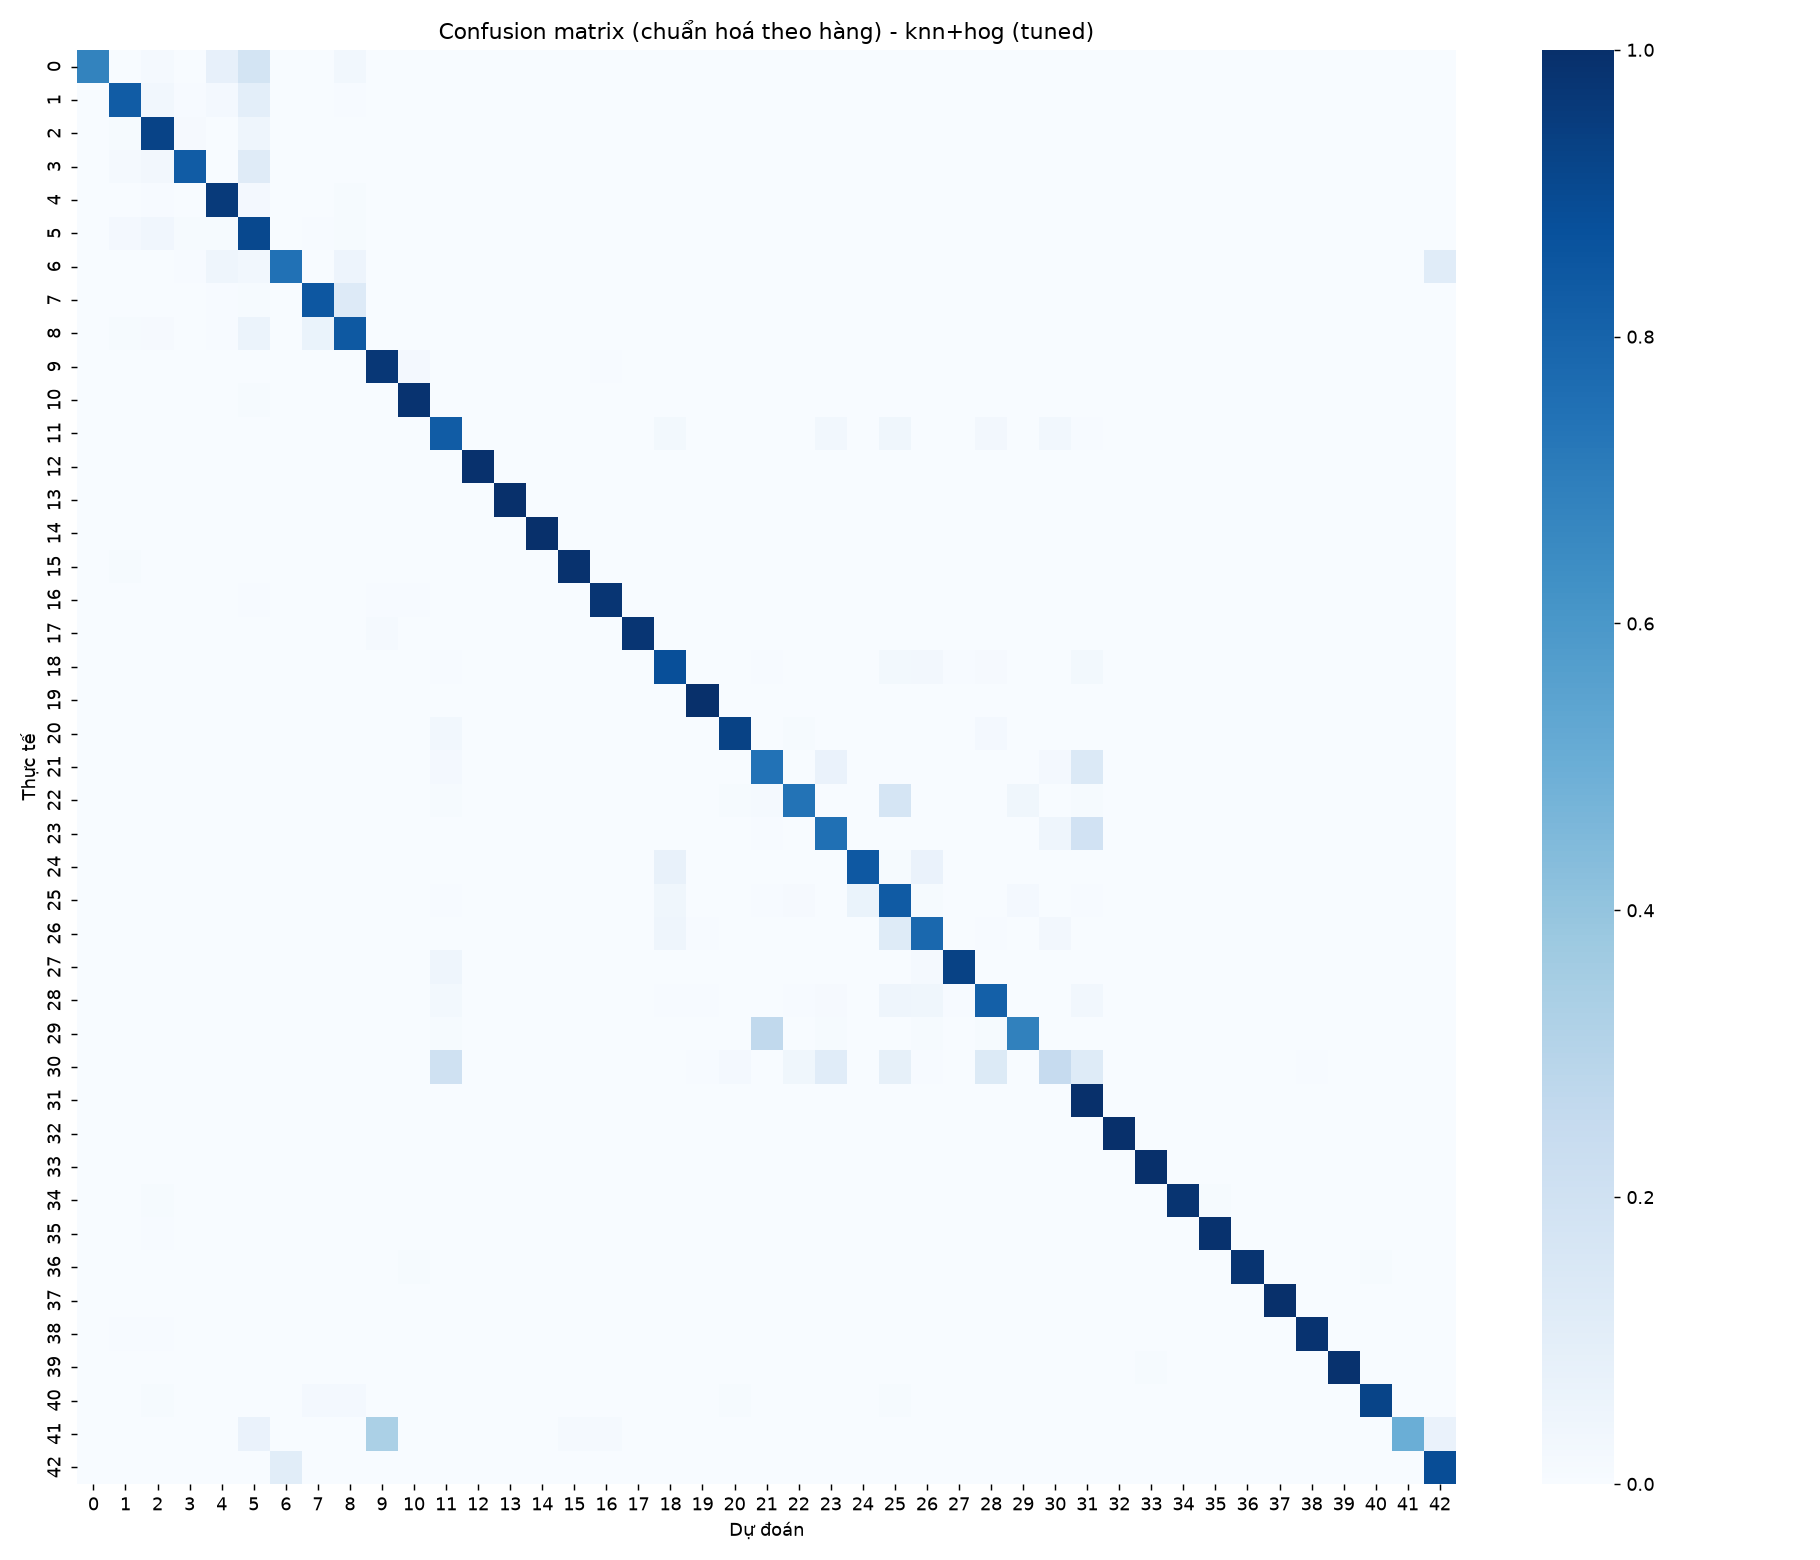
\includegraphics[width=0.8\textwidth]{images/fig_confusion_best.png}
    \caption{Ma trận nhầm lẫn (chuẩn hóa theo hàng) của K-NN kết hợp HOG trên tập Test}
    \label{fig:ma-tran-nham-lan}
    \Nguon{Nhóm vẽ từ kết quả thực nghiệm}
\end{figure}

\begin{table}[H]
\centering
\caption{Mười cặp lớp bị nhầm lẫn nhiều nhất trên tập Test}
\label{tab:cap-nham-lan}
\begin{tabular}{|c|p{5.4cm}|p{6.6cm}|}
\hline
\textbf{Số ảnh} & \textbf{Lớp thực tế} & \textbf{Lớp được dự đoán} \\
\hline
72 & 1 -- Speed limit 30 & 5 -- Speed limit 80 \\
\hline
59 & 7 -- Speed limit 100 & 8 -- Speed limit 120 \\
\hline
55 & 3 -- Speed limit 60 & 5 -- Speed limit 80 \\
\hline
34 & 2 -- Speed limit 50 & 5 -- Speed limit 80 \\
\hline
31 & 30 -- Beware ice/snow & 11 -- Right-of-way at intersection \\
\hline
31 & 25 -- Road work & 24 -- Road narrows on right \\
\hline
29 & 23 -- Slippery road & 31 -- Wild animals crossing \\
\hline
29 & 8 -- Speed limit 120 & 7 -- Speed limit 100 \\
\hline
28 & 8 -- Speed limit 120 & 5 -- Speed limit 80 \\
\hline
24 & 29 -- Bicycles crossing & 21 -- Double curve \\
\hline
\end{tabular}
\Nguon{Nhóm tổng hợp từ tệp \texttt{results/top\_confusions.csv}}
\end{table}

\begin{table}[H]
\centering
\caption{Các lớp có F1 thấp nhất và cao nhất của mô hình tốt nhất trên tập Test}
\label{tab:f1-theo-lop}
\begin{tabular}{|c|p{7.6cm}|c|c|}
\hline
\textbf{Lớp} & \textbf{Tên lớp} & \textbf{F1} & \textbf{Số ảnh Test} \\
\hline
30 & Beware ice/snow & 0.350 & 150 \\
\hline
41 & End of no passing & 0.667 & 60 \\
\hline
21 & Double curve & 0.713 & 90 \\
\hline
29 & Bicycles crossing & 0.734 & 90 \\
\hline
23 & Slippery road & 0.746 & 150 \\
\hline
13 & Yield & 0.999 & 720 \\
\hline
32, 37 & End of all speed/passing limits; Go straight or left & 1.000 & 60 \\
\hline
\end{tabular}
\Nguon{Nhóm tổng hợp từ tệp \texttt{results/per\_class\_f1.csv}}
\end{table}

\begin{table}[H]
\centering
\caption{Độ chính xác của K-NN kết hợp HOG theo cạnh nhỏ nhất của ảnh gốc (tập Test)}
\label{tab:theo-kich-thuoc}
\begin{tabular}{|p{5.5cm}|p{3.5cm}|p{3.5cm}|}
\hline
\textbf{Cạnh nhỏ nhất (điểm ảnh)} & \textbf{Số ảnh} & \textbf{Accuracy} \\
\hline
Từ 30 trở xuống & 1\,811 & 0.8382 \\
\hline
Trên 30 đến 40 & 4\,098 & 0.8997 \\
\hline
Trên 40 đến 60 & 4\,202 & 0.9260 \\
\hline
Trên 60 đến 100 & 1\,979 & 0.9444 \\
\hline
Trên 100 & 540 & 0.9352 \\
\hline
\end{tabular}
\Nguon{Nhóm tổng hợp từ tệp \texttt{results/accuracy\_by\_size.csv}}
\end{table}

\begin{figure}[H]
    \centering
    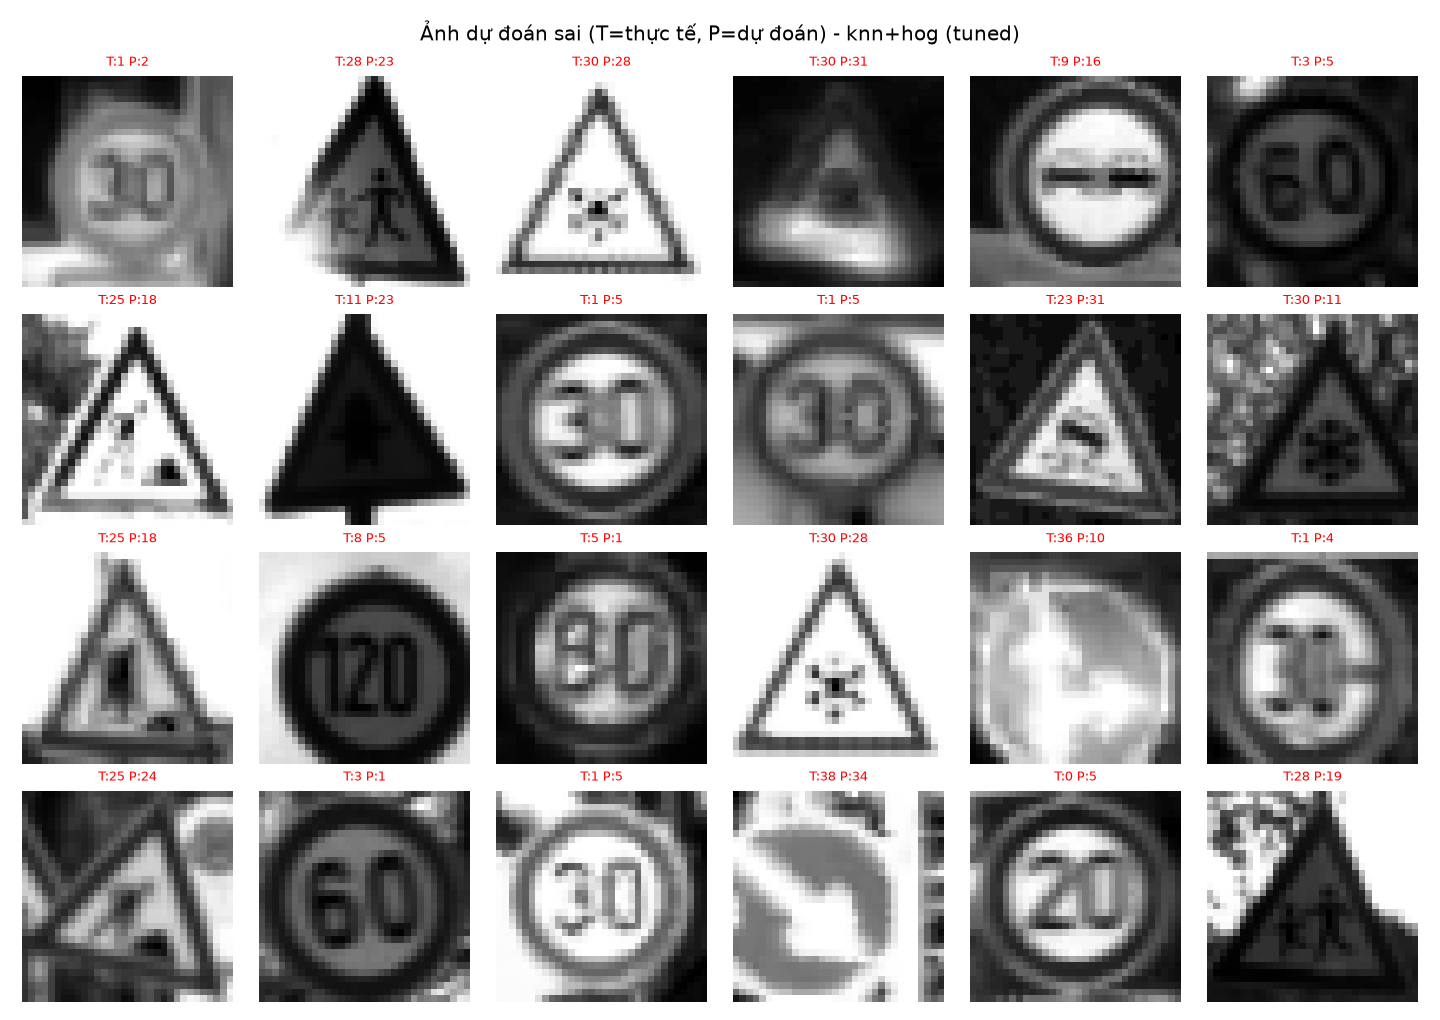
\includegraphics[width=0.8\textwidth]{images/fig_errors.png}
    \caption{24 ảnh Test bị dự đoán sai (T: nhãn thực, P: nhãn dự đoán), lấy ngẫu nhiên}
    \label{fig:anh-du-doan-sai}
    \Nguon{Nhóm vẽ từ kết quả thực nghiệm}
\end{figure}

\section{Thảo luận và so sánh}

\subsection{So sánh các phương án}

\textbf{Biểu diễn đặc trưng.} HOG vượt trội pixel với cả hai thuật toán: K-NN đạt Macro-F1 0.8840 (HOG) so với 0.6667 (pixel đã chọn tham số), Cây quyết định đạt 0.6887 so với 0.6356. Một cách giải thích hợp lý là HOG mô tả hướng của đường biên và hình dạng cục bộ, ít phụ thuộc vào độ sáng tuyệt đối, trong khi khoảng cách giữa hai vector pixel bị chi phối bởi độ sáng \textit{(giả thuyết của nhóm, chưa kiểm chứng riêng)}. Quan sát ở Bảng~\ref{tab:clahe} phù hợp với cách giải thích này: CLAHE giúp biểu diễn pixel rất nhiều nhưng gần như không đổi với HOG.

\textbf{Tác động của PCA.} Với HOG, PCA giảm số chiều từ 1\,764 xuống 100 mà gần như không làm mất độ chính xác (K-NN: Accuracy 0.9051 so với 0.9082) và giảm thời gian dự đoán từ 147,05 giây xuống 62,88 giây. Với pixel, PCA lại \textit{tăng} chất lượng K-NN (0.7683 so với 0.7051); một cách giải thích có thể là PCA giữ các hướng biến thiên chính và loại bớt nhiễu điểm ảnh \textit{(giả thuyết)}. Ngược lại, PCA làm Cây quyết định kém đi ở cả hai biểu diễn (pixel: 0.7130 xuống 0.5793; HOG: 0.7595 xuống 0.7166), có thể vì các thành phần chính trộn nhiều đặc trưng gốc nên phép chia theo một trục kém hiệu quả hơn \textit{(giả thuyết)}.

\textbf{K-NN so với Cây quyết định.} Ở cùng biểu diễn HOG, K-NN hơn Cây quyết định khoảng 15 điểm phần trăm Accuracy (0.9082 so với 0.7595). Cây quyết định chọn từng ngưỡng trên một đặc trưng, trong khi bài toán có 43 lớp và vector đặc trưng nhiều chiều với nhiều lớp khá giống nhau; K-NN so sánh toàn bộ vector \textit{(giả thuyết)}. Hai thuật toán cũng đối lập về chi phí: Cây quyết định mất 388,59 giây để huấn luyện trên HOG nhưng chỉ 0,37 giây để dự đoán, còn K-NN gần như không tốn thời gian huấn luyện (0,14 giây) nhưng mất 147,05 giây để dự đoán 12\,630 ảnh so với toàn bộ 39\,209 ảnh huấn luyện.

\textbf{Kiểm định và kiểm thử.} K-NN kết hợp HOG đạt Accuracy 0.9284 trên tập kiểm định nhưng 0.9082 trên tập Test. Chênh lệch khoảng 2 điểm phần trăm là hợp lý vì Test gồm các track hoàn toàn khác; điều này cho thấy việc chia kiểm định theo track giữ cho ước lượng không quá lạc quan.

\subsection{Phân tích các dự đoán sai}

\textbf{Biển giới hạn tốc độ.} Các cặp bị nhầm nhiều nhất đều là biển giới hạn tốc độ (Bảng~\ref{tab:cap-nham-lan}): lớp 1 bị dự đoán thành lớp 5 (72 ảnh), lớp 7 thành lớp 8 (59 ảnh), lớp 3 thành lớp 5 (55 ảnh). Các biển này cùng hình dạng, cùng viền đỏ và chỉ khác ở chữ số bên trong; ở độ phân giải $32\times32$ các chữ số rất nhỏ nên dễ bị lẫn \textit{(giả thuyết, cần đối chiếu với các ảnh trong Hình~\ref{fig:anh-du-doan-sai})}. Xét về ứng dụng, lỗi nghiêm trọng nhất là dự đoán giới hạn cao hơn giới hạn thực (từ 30 lên 80 km/h), vì có thể khiến hệ thống cho phép tốc độ không an toàn.

\textbf{Biển cảnh báo hình tam giác.} Lớp 30 (Beware ice/snow) có F1 thấp nhất (0.350) và hay bị nhầm với lớp 11 (Right-of-way at intersection). Các cặp (25, 24), (23, 31), (29, 21) cũng đều là biển tam giác viền đỏ có hình minh họa nhỏ ở giữa, nên khác biệt chủ yếu nằm ở chi tiết bên trong \textit{(giả thuyết)}. Các lớp có hình dạng riêng biệt như Yield (lớp 13, F1 bằng 0.999) hầu như không bị sai.

\textbf{Kích thước biển.} Độ chính xác giảm khi ảnh nhỏ: 0.8382 với cạnh nhỏ nhất từ 30 điểm ảnh trở xuống so với 0.9444 ở nhóm trên 60 đến 100 điểm ảnh (Bảng~\ref{tab:theo-kich-thuoc}). Biển nhỏ (ở xa) mất nhiều chi tiết hơn khi đổi kích thước, phù hợp với phân tích lỗi ở trên. Nhóm trên 100 điểm ảnh (540 ảnh) có độ chính xác 0.9352, thấp hơn nhóm trên 60 đến 100 một chút nhưng số mẫu nhỏ nên chưa đủ để kết luận.

\subsection{Hạn chế}
\label{sec:han-che}

\begin{itemize}
    \item \textbf{Mất thông tin màu} do chuyển sang ảnh xám; màu là dấu hiệu quan trọng của biển báo.
    \item \textbf{Độ phân giải thấp} ($32\times32$) làm mất chi tiết chữ số và hình minh họa nhỏ, là nguyên nhân khả dĩ của các cặp nhầm lẫn chính.
    \item \textbf{Phụ thuộc ROI:} mô hình dùng khung biển có sẵn trong tệp CSV; ngoài thực tế cần bộ phát hiện biển.
    \item \textbf{Chỉ một lần chia kiểm định} (một phần trong 5 phần), chưa dùng đánh giá chéo đầy đủ nên chưa có khoảng tin cậy cho các chênh lệch nhỏ (ví dụ giữa K-NN kết hợp HOG và K-NN kết hợp PCA-HOG: 0.9082 và 0.9051).
    \item \textbf{Chọn mô hình cho phân tích lỗi:} mã nguồn chọn mô hình tốt nhất theo Macro-F1 trên tập Test (\texttt{02\_experiments.py}, mục 6). Cấu hình này cũng đứng đầu trên tập kiểm định nên kết luận không đổi, nhưng đúng quy trình hơn là chọn theo tập kiểm định.
    \item \textbf{K-NN dự đoán chậm} và phải lưu toàn bộ dữ liệu huấn luyện, khó dùng cho ứng dụng thời gian thực.
    \item \textbf{Phạm vi dữ liệu:} GTSRB chỉ gồm biển báo của Đức, không đảm bảo kết quả trên biển báo Việt Nam.
\end{itemize}
